% ==========================================
% CHAPTER 1: Theory
% ==========================================
\chapter{Introduction to the Internet of Things}

\textbf{In This Chapter:}
\begin{itemize}
    \item Understanding the scale of the IoT Revolution.
    \item The critical hardware constraints defining edge devices.
\end{itemize}

The Internet of Things (IoT) seamlessly blends the physical and digital worlds. A microchip costing less than a dollar can now read real-world data—temperature, pressure, heart rate, or industrial fluid flow—and transmit it globally across the internet. 

\section{The Architectural Flaw of IoT}
Why do we need a dedicated class for IoT security? Because IoT devices differ fundamentally from the desktop computers or smartphones we use daily. 

A modern PC has an incredibly complex operating system (like Windows 11), hardware-enforced memory isolation, and layers of dedicated antivirus software. Conversely, an IoT microcontroller possesses minimal kilobytes of memory and runs a single loop of compiled code bare-metal on the silicon. It communicates natively over TCP/IP sockets without a protective firewall wrapper. If your code tells the web server to accept a malicious query, the silicon obeys instantly. There is no software fail-safe beneath your code.

% ==========================================
% CHAPTER 2: Security
% ==========================================
\chapter{Introduction to Cyber Security in IoT}

\textbf{In This Chapter:}
\begin{itemize}
    \item Defining the CIA Triad (Confidentiality, Integrity, Availability).
    \item Modeling automated vs.\ manual threat actors.
\end{itemize}

\section{The CIA Triad}
Whenever you design an IoT system, you must systematically grade it against these three pillars:
\begin{itemize}
    \item \textbf{Confidentiality:} Ensuring data is only accessible to authorized viewers. (e.g., utilizing WPA2/WPA3 Wi-Fi encryption over open airspace).
    \item \textbf{Integrity:} Assuring that data is accurate and unchanged. This is arguably the most critical pillar for industrial IoT. If a sensor reads the temperature of a data center server rack, we must be absolutely certain that a hacker cannot inject a "fake" reading of 999 degrees Celsius. We will exploit a devastating lack of integrity heavily in Chapter 5.
    \item \textbf{Availability:} Guaranteeing that systems are available to users. Because IoT processors are slow, they are uniquely susceptible to Denial of Service (DoS) attacks.
\end{itemize}

% ==========================================
% CHAPTER 3: Hardware & Setup
% ==========================================
\chapter{Meet the Hardware Platforms \& IDE Setup}

\textbf{In This Chapter:}
\begin{itemize}
    \item Step-by-step environment setup for Arduino IDE (C++).
    \item Step-by-step firmware flashing and Thonny SDK for the Pico W.
    \item Official documentation web links.
\end{itemize}

To master both foundational embedded programming and modern rapid prototyping, this book features two parallel architectures.

\section{NodeMCU (ESP8266)}
The NodeMCU, utilizing the ESP8266 silicon, defined the maker-IoT revolution. It features a 32-bit RISC CPU running at 80 MHz with heavily integrated Wi-Fi capabilities. Because of its legendary status, it possesses arguably the largest open-source C++ library ecosystem in the world for an IoT device. Learn more at the official Espressif website: \url{https://www.espressif.com/en/products/socs/esp8266}.

\begin{figure}[h]
    \centering
    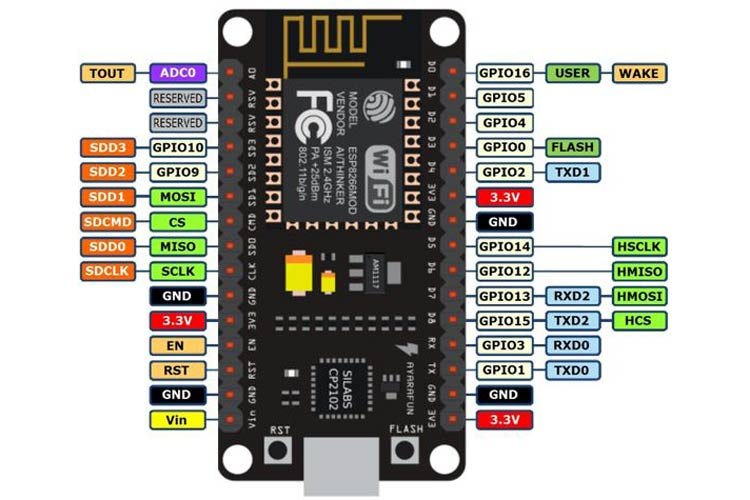
\includegraphics[width=0.9\textwidth]{NodeMCU-ESP8266-Pinout.jpg}
    \caption{NodeMCU ESP8266 Pinout Mapping}
\end{figure}

\subsection{Connecting \& Setup: Arduino IDE}
\textbf{Step 1:} Download the Arduino IDE from \url{https://arduino.cc}. \\
\textbf{Step 2:} Open the IDE and navigate to \textbf{File > Preferences}. \\
\textbf{Step 3:} In the \textit{Additional Boards Manager URLs} box, exactly paste: \\ \texttt{http://arduino.esp8266.com/stable/package\_esp8266com\_index.json} \\
\textbf{Step 4:} Go to \textbf{Tools > Board > Boards Manager}. Search for \texttt{esp8266} and Install the package. \\
\textbf{Step 5:} Connect the NodeMCU to your computer via USB (Ensure the cable supports Data Transfer). \\
\textbf{Step 6:} Go to \textbf{Tools > Port} and select the active COM port. Select \textbf{Tools > Board > NodeMCU 1.0}.

\begin{troubleshootbox}[Arduino IDE: Port Not Showing Up]
1. Swap the USB cable. Charging cables lack the D+ / D- internal data lines needed for communication. \\
2. Install the CH340 or CP2102 Serial Drivers if you are on an older Windows or Mac OS.
\end{troubleshootbox}

\section{Raspberry Pi Pico W}
The Pico W is a massive architectural leap. It is driven by the RP2040 chip—a custom dual-core Arm Cortex-M0+ running at 133 MHz, paired with an Infineon wireless module. Because of its processing power, it is capable of running an entire Python Interpreter natively on bare metal. Official Datasheet: \url{https://datasheets.raspberrypi.com/picow/pico-w-datasheet.pdf}.

\begin{figure}[h]
    \centering
    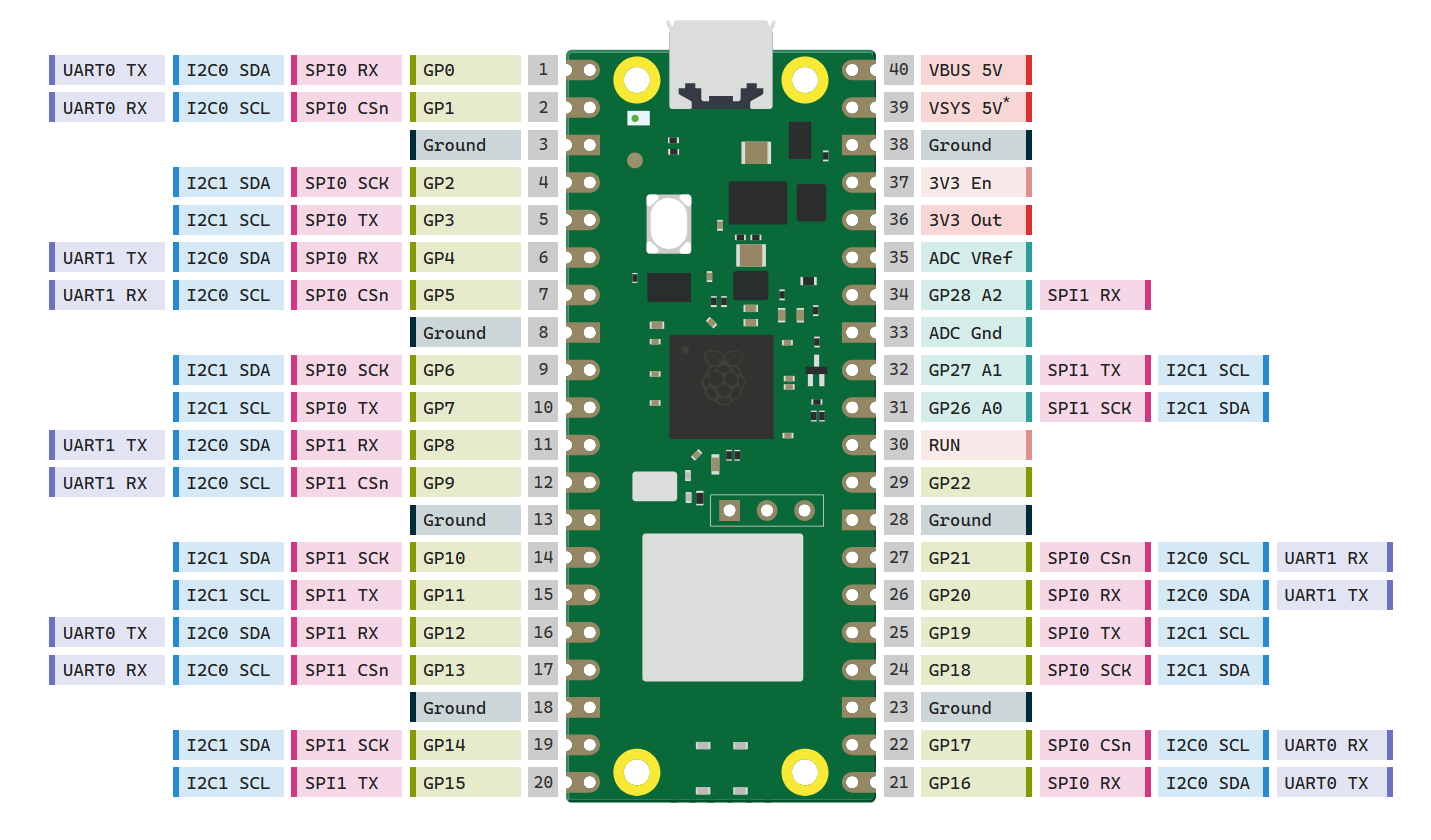
\includegraphics[width=0.9\textwidth]{Raspberry_Pi_Pico_W.png}
    \caption{Raspberry Pi Pico W Pinout Mapping}
\end{figure}

\subsection{Connecting \& Setup: Thonny IDE}
\textbf{Step 1:} Download the Thonny Python IDE from \url{https://thonny.org}. \\
\textbf{Step 2:} Hold down the tiny \texttt{BOOTSEL} button on the physical board while inserting the USB cable. Release after inserting. It will mount on your PC like a USB drive named \texttt{RPI-RP2}. \\
\textbf{Step 3:} Download the MicroPython UF2 firmware file from \url{https://micropython.org/download/rp2-pico-w/}. Drag and drop this `.uf2` file into the \texttt{RPI-RP2} drive. The drive will disappear as the board reboots. \\
\textbf{Step 4:} Open Thonny. In the bottom right corner, click the interpreter label and strictly select \textbf{MicroPython (Raspberry Pi Pico)}. \\
\textbf{Step 5:} Write code in the editor, press "Save", and select the Pico internal storage to save files permanently.

\begin{troubleshootbox}[Thonny: "OSError: Device is Busy"]
MicroPython runs a continuous REPL loop. If you deploy an infinite loop (`while True:`) without `time.sleep()` delays, the CPU hits 100\% utilization and locks the USB interface. \\
\textbf{The Fix:} Mash the red "STOP" sign in Thonny 5-6 times rapidly to force a `KeyboardInterrupt` over the serial hardware, breaking the loop safely.
\end{troubleshootbox}
